%!TEX encoding = UTF-8 Unicode
% coding: utf-8

%!TEX encoding = UTF-8 Unicode
% coding: utf-8
% Header per le presentazioni in LaTeX+beamer
% @author Eric Miotto
% @date 15/12/2006

\documentclass{beamer}

%Configurazione beamer
\mode<presentation>
{
 %Tema grafico
  \usetheme{Frankfurt}
  
  %Colori da usare per il tema
  \usecolortheme{seahorse} 
  \usecolortheme{rose} 

  \setbeamercovered{transparent}
}

%Importazione package
\usepackage[italian]{babel} %Lingua e sillabazione in italiano
\usepackage[utf8]{inputenc} %Codifica UTF8
\usepackage{textpos} %Posizionamento testo e immagini ovunque sulla pagina

% Griglia di posizionamento delle immagini
% Il primo parametro sono il numero di colonne in cui viene diviso il foglio,
% il secondo sono il numero di righe in cui viene diviso il foglio
%\TPGrid{3}{1}

\title{Presentazione Campagna di Qualifica \\ per C04}

\author{Egoless Group}

\date[RQ 21/03/2007] % (optional, should be abbreviation of conference name)
{Revisione di Qualifica \\ 21 marzo 2007}

\subject{Presentazione della definizione di prodotto per il capitolato C04}

\logo{
\includegraphics[width=1cm]{img/logo.jpg}}

% Delete this, if you do not want the table of contents to pop up at
% the beginning of each subsection:

%Ci pensa lui a creare l'indice

%\AtBeginSubsection[]
%{
%  \begin{frame}<beamer>
%    \frametitle{Outline}
%    \tableofcontents[currentsection,currentsubsection]
%  \end{frame}
%}

\AtBeginSection[]
{
  \begin{frame}<beamer>
    \frametitle{Outline}
    \tableofcontents[currentsection]
  \end{frame}
}

\begin{document}

\begin{frame}
  \titlepage
\end{frame}

\begin{frame}
  \frametitle{Outline}
  \tableofcontents
  % You might wish to add the option [pausesections]
\end{frame}


% Structuring a talk is a difficult task and the following structure
% may not be suitable. Here are some rules that apply for this
% solution: 

% - Exactly two or three sections (other than the summary).
% - At *most* three subsections per section.
% - Talk about 30s to 2min per frame. So there should be between about
%   15 and 30 frames, all told.

% - A conference audience is likely to know very little of what you
%   are going to talk about. So *simplify*!
% - In a 20min talk, getting the main ideas across is hard
%   enough. Leave out details, even if it means being less precise than
%   you think necessary.
% - If you omit details that are vital to the proof/implementation,
%   just say so once. Everybody will be happy with that.

\section{Conduzione del progetto}

\subsection*{Conduzione del progetto}

\begin{frame}
\frametitle{Rapporti con il prof. Zambello}

\begin{itemize}
\item abbiamo concordato la visita dell'istituto per geometri Belzoni per martedì 27 marzo
\end{itemize}

\end{frame}

\begin{frame}
\frametitle{Collaborazione con Swell Systems}

\begin{itemize}
\item presi accordi circa le interfacce
\item per l'integrazione si discuterà più avanti
\end{itemize}

\end{frame}

\begin{frame}
\frametitle{Pianificazione}

\begin{figure}
  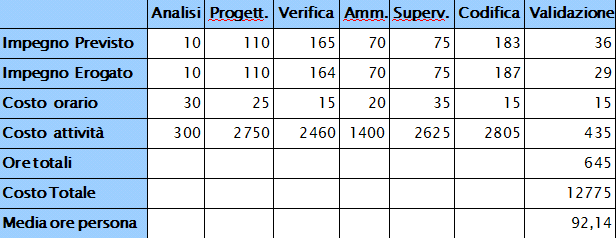
\includegraphics[width=10cm]{img/Consuntivo.png}
\end{figure}

\end{frame}

\begin{frame}
\frametitle{Pianificazione}

\begin{figure}
  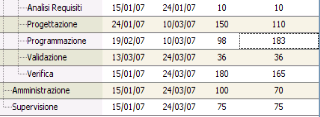
\includegraphics[width=10cm]{img/AdeguamentoOreGantt.png}
\end{figure}

\end{frame}

\begin{frame}
\frametitle{Pianificazione}

\begin{figure}
  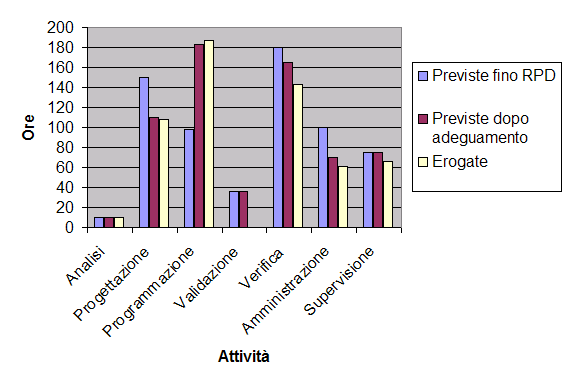
\includegraphics[width=10cm]{img/Previste_Erogate.png}
\end{figure}

\end{frame}

\begin{frame}
\frametitle{Considerazione sul manuale utente}

\begin{itemize}
\item è stata consegnata una prima bozza del manuale utente
\item il prodotto impatta però sui processi della scuola
\item il manuale utente da solo non basta, bisogna organizzare del training per l'uso del prodotto
\end{itemize}

\end{frame}

\section{Campagna di qualifica}

\subsection*{Campagna di qualifica}

\begin{frame}
\frametitle{Cosa abbiamo testato}

\begin{itemize}
	\item i Web Service in WSDidattica
	\item i bean in APPDidattica
	\item la GUI di APPDidattica non è stata per ora testata (dobbiamo investigare sui metodi per farlo)
\end{itemize}
\end{frame}

\begin{frame}
\frametitle{Schema generale dei test}

\begin{figure}
  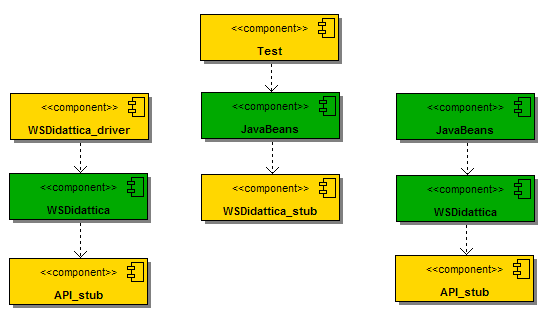
\includegraphics[width=10cm]{img/SchemaGeneraleTest.png}
\end{figure}

\end{frame}

\begin{frame}
\frametitle{Test di WSDidattica}
\begin{itemize}
\item avevamo già realizzato API\_Stub per simulare i componenti forniti da Swell e il modo in cui dovremmo lavorare
\item lo abbiamo esteso per avere un minimo di persistenza e per poterne pilotare lo stato (con un ulteriore WS)
\item WSDidattica si appoggia a questo e viene pilotato da un driver che contiene i test
\item per la natura del componente non è previsto nessun test strutturale
\end{itemize}

\end{frame}

\begin{frame}
\frametitle{Test di WSDidattica}
\framesubtitle{Esiti}

\begin{itemize}
\item risultati positivi
\item testati anche le eccezioni previste (sono state sollevate correttamente)
\end{itemize}

\end{frame}

\begin{frame}
\frametitle{Test di APPDidattica}
\begin{itemize}
\item realizzato uno stub di WSDidattica, che offre
\begin{itemize}
\item la persistenza necessaria ai test
\item un WS per pilotare il suo stato
\end{itemize}

\item i test sono stati messi direttamente in APPDidattica
\item in APPDidattica c'è un client per lo stub che serve solo per i test
\end{itemize}

\end{frame}

\begin{frame}
\frametitle{Test di APPDidattica}
\framesubtitle{Esiti}

\begin{itemize}
\item con i test funzionali si sono scoperti un bel po' di comportamenti errati
\begin{itemize}
\item dovuti a assunzioni sbagliate su altri oggetti usati
\item dovuti a non adesione alle specifiche date
\end{itemize}

\item i test di copertura, che usano i test funzionali, hanno coperto codice  e cammini in maniera soddisfacente
\begin{itemize}
\item 100\% branch coverage, $>$75\% line coverage
\end{itemize}

\end{itemize}

\end{frame}

\begin{frame}
\frametitle{Qualche considerazione}

\begin{itemize}
\item abbiamo constatato come fare test sia costoso
\begin{itemize}
\item richiedono progettazione attenta (a tratti ci sembrava di rifare la parte di Swell!)
\item richiedono molto tempo per essere codificati
\item il tempo di esecuzione risulta essere risibile grazie all'automazione che siamo riusciti ad attuare
\end{itemize}

\item e\ldots non li abbiamo pianificati a sufficienza
\end{itemize}


\end{frame}

\begin{frame}
\frametitle{Verifica dei processi}

\begin{itemize}
\item Primari
	\begin{itemize}
		\item Fornitura: gestione difficoltosa dei rapporti con il cliente in graduale miglioramento
		\item Sviluppo: soppressione iterazione ma corretta ripartizione ruoli e compiti
	\end{itemize}
	\item Di Supporto
	\begin{itemize}
		\item Documentazione: il rispetto delle norme tempestivamente stese ha garantito documenti ben formati
		\item Verifica: tempestiva per i documenti; in ritardo per il codice.
	\end{itemize}
\end{itemize}




\end{frame}

\section{Cosa abbiamo sbagliato finora}

\subsection*{Cosa abbiamo sbagliato finora}

\begin{frame}
\frametitle{Cosa abbiamo sbagliato finora}

\begin{quote}
much design work is performed within the construction activity itself
\end{quote}

\begin{flushright}
SWEBOK
\end{flushright}

\begin{itemize}
\item progettazione di dettaglio fatta senza mettere mano al codice
\begin{itemize}
\item abbiamo poi scoperto dei problemi che ci hanno fatto ripensare ad alcune scelte
\end{itemize}

\item verifica del codice sottovalutata come impegno
\end{itemize}

\end{frame}

\end{document}